\documentclass [oneside] {article}

% Letter size, to match the pages of the book.
\usepackage [papersize={8.5in,11in}, margin=0in] {geometry}
\usepackage {tikz}
\usepackage {xcolor}

\usepackage [T1] {fontenc}
\usepackage {newpxtext}
\usepackage [vvarbb,cmintegrals,cmbraces,bigdelims] {newpxmath}

\usepackage {graphicx}

\begin {document}
\thispagestyle{empty}
\tikz[remember picture, overlay] \node  at (current page.center)%
	{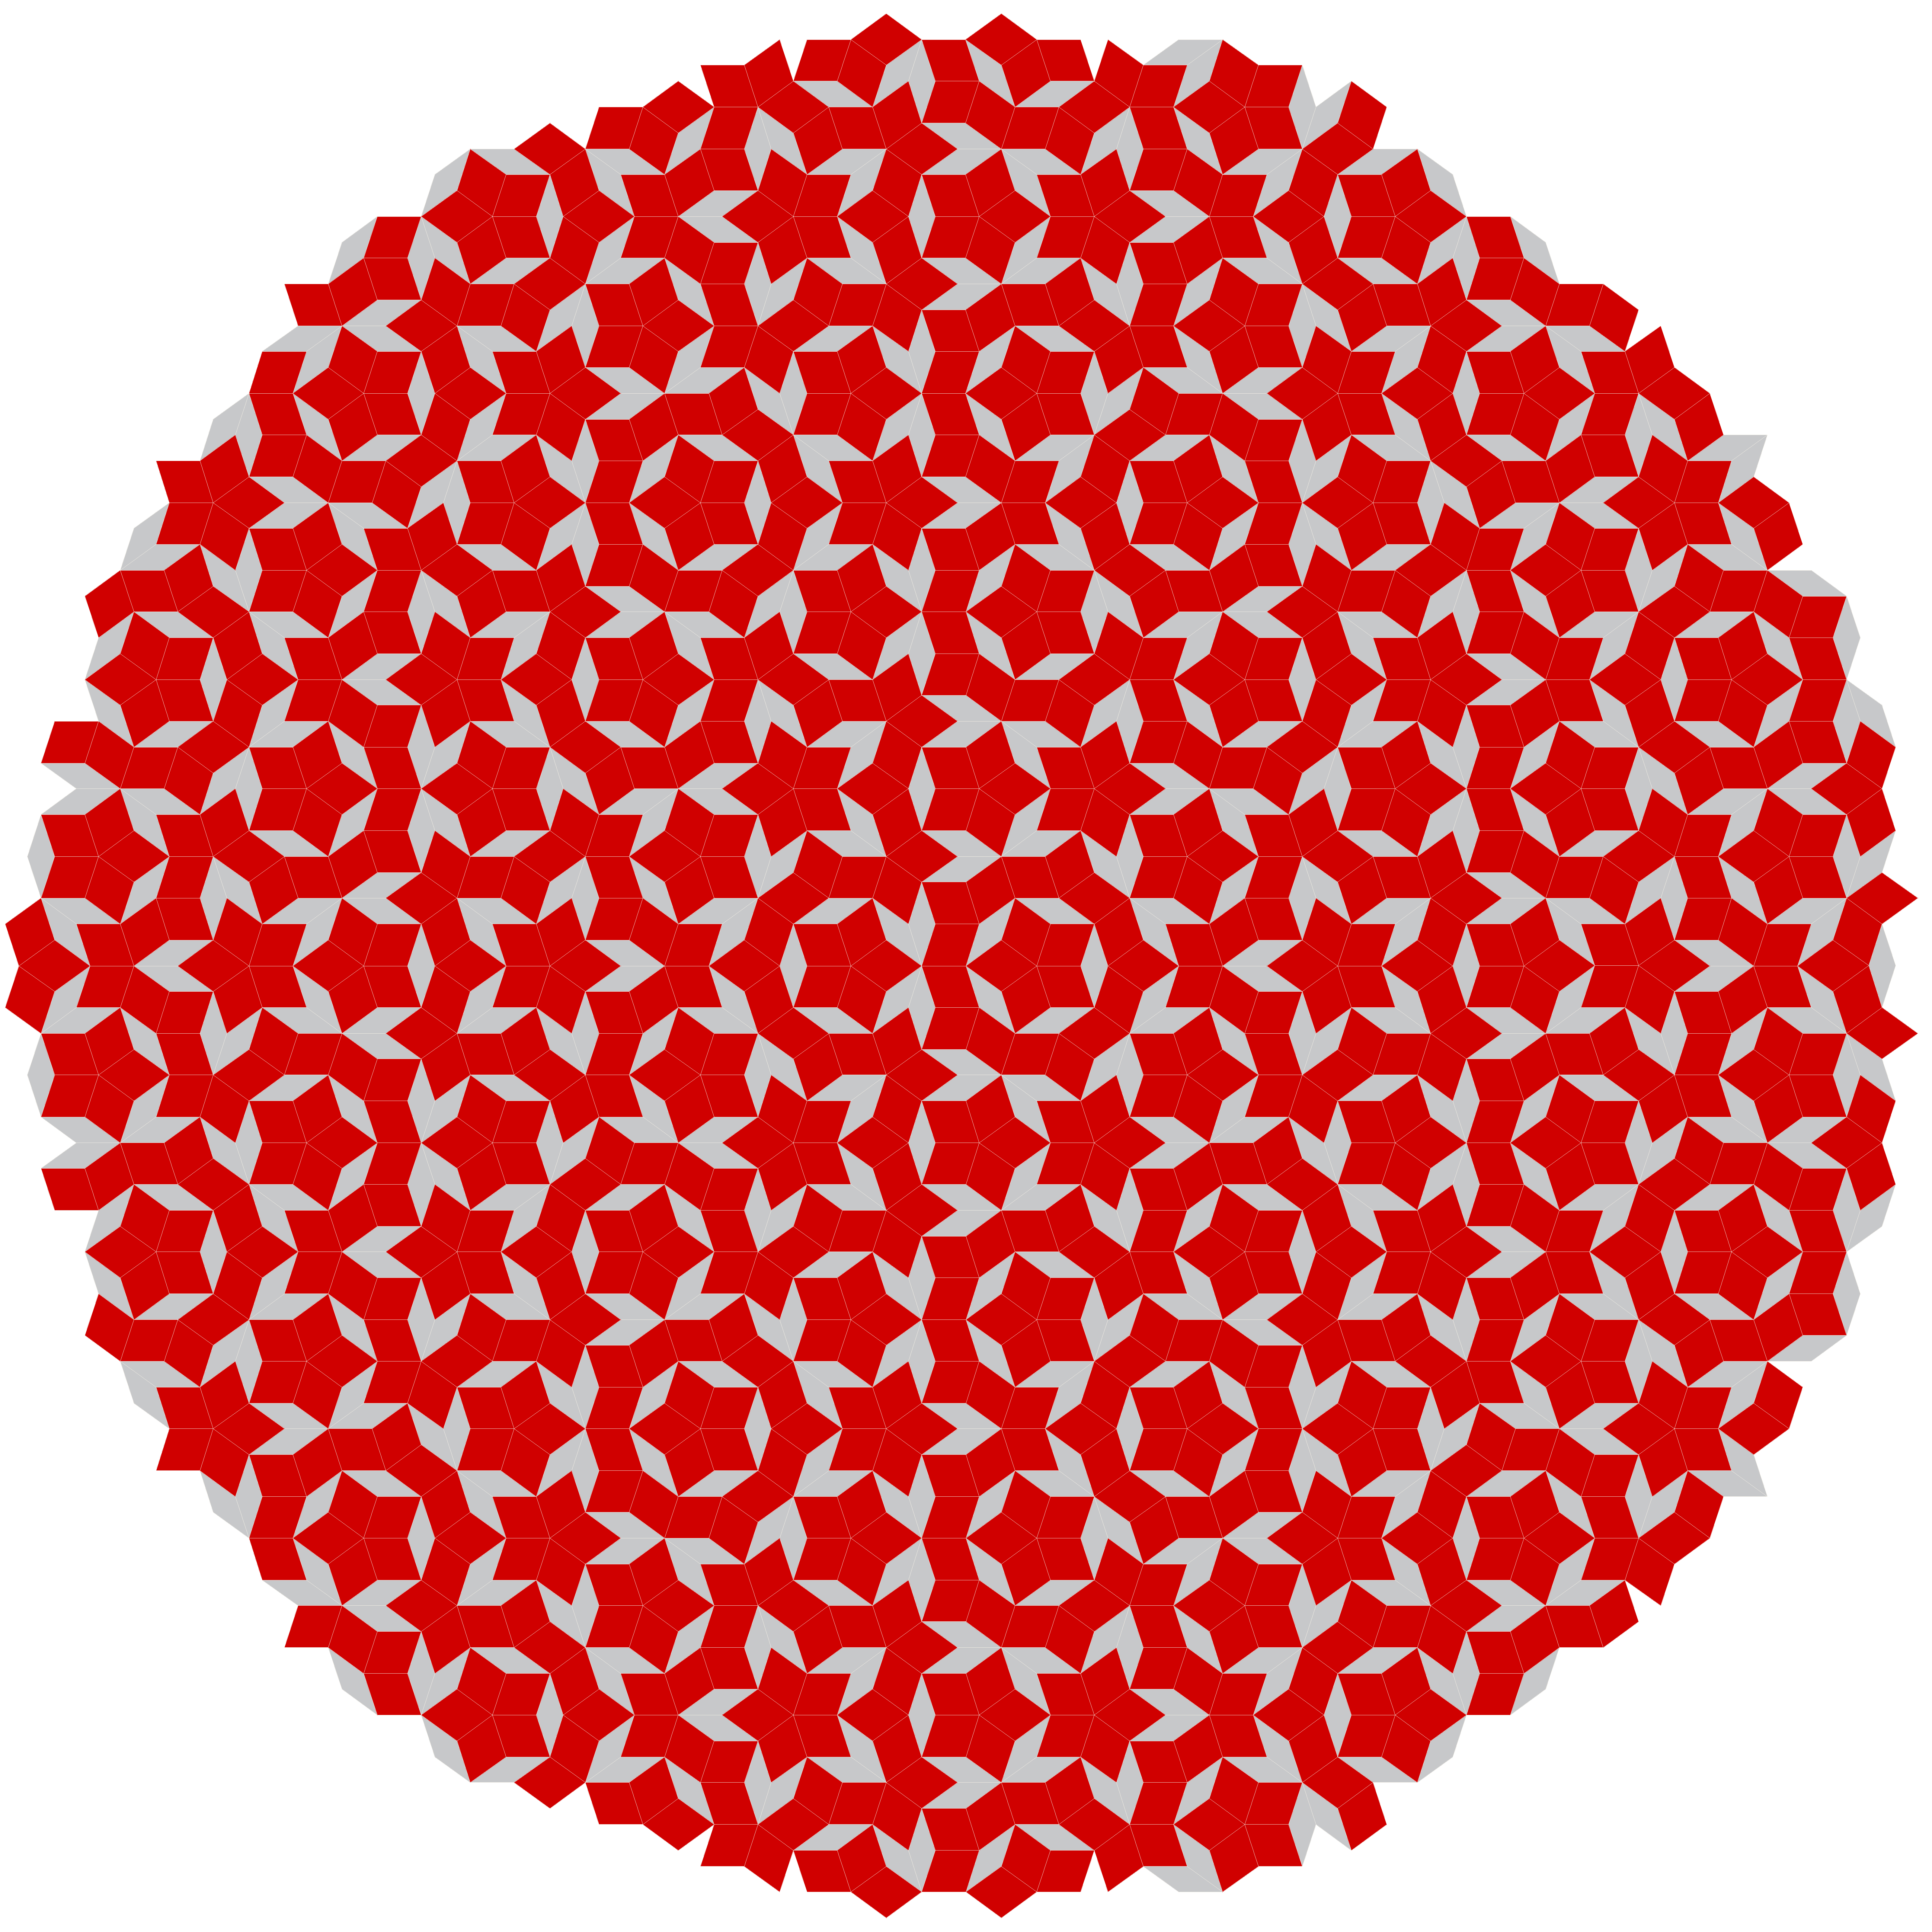
\includegraphics [scale=0.49] {penrose}};

\vspace {\stretch{2}}

\noindent
\begin {center}

\begin{tikzpicture}
	\fill [fill=white, fill opacity = 0.8, rounded corners = 1ex]
		(0,0) rectangle (16,6) ;
	\node [align=center, font=\fontsize{26pt}{26pt}\scshape] at (8,4.2)
		{Coordinated Linear Algebra} ;
	\node [align=center, font=\fontsize{17pt}{17pt}\scshape] at (8,1.8)
		{2026--2027} ;
  \end{tikzpicture}
\end {center}

\vspace {\stretch{3}}
\end {document}
